\documentclass[10pt,journal,compsoc]{IEEEtran}
\usepackage[utf8]{inputenc}
\usepackage{amsmath,amsfonts,amssymb}
\usepackage{graphicx}
\usepackage{booktabs}
\usepackage{array}
\usepackage{microtype}
\usepackage[hidelinks]{hyperref}
\usepackage{cite}
\usepackage{textcomp}
\usepackage{float}
\usepackage{dblfloatfix}
\usepackage{placeins}

\graphicspath{{../output/paper/figures/}}
\hypersetup{colorlinks=false, pdfborder={0 0 0}}

% Every result quoted in the text is a macro generated by research/reproduce_all.py.
% Generated by research/reproduce_all.py -- do not edit by hand.
\newcommand{\HeadlineReturn}{49.57}
\newcommand{\HeadlineTrades}{67}
\newcommand{\HeadlineSharpe}{2.07}
\newcommand{\ClosedFormReturn}{36.63}
\newcommand{\ClosedFormTrades}{66}
\newcommand{\ForwardReturn}{5.01}
\newcommand{\ForwardTrades}{15}
\newcommand{\LagReturn}{0.17}
\newcommand{\LockReturn}{3.92}
\newcommand{\LockTrades}{3}
\newcommand{\FullChainDReturn}{-44.41}
\newcommand{\FullChainDTrades}{29}
\newcommand{\GridErrMean}{1.70}
\newcommand{\GridErrMax}{10.83}
\newcommand{\GridErrShare}{42.9}
\newcommand{\GridSpearman}{-0.9997}
\newcommand{\ParityResidualMean}{15.84}
\newcommand{\AtmPutBias}{-11.28}
\newcommand{\AtmCallBias}{4.57}
\newcommand{\HeadlineSharpeMTM}{1.85}
\newcommand{\HeadlineMDDStep}{11.61}
\newcommand{\HeadlineMDDMTM}{15.07}
\newcommand{\PriceFieldMismatch}{55.5}
\newcommand{\PriceFieldMismatchTraded}{18.9}
\newcommand{\CellsPositive}{3}
\newcommand{\CellsCIAboveZero}{0}
\newcommand{\HybridAReturn}{25.7}
\newcommand{\HybridAExMax}{4.3}
\newcommand{\PureDReturn}{-44.4}
\newcommand{\PureDExMax}{-9.3}
\newcommand{\PureDLargest}{35,133}
\newcommand{\HybridAPctl}{93}
\newcommand{\RetailDReturn}{2.1}
\newcommand{\RetailDExMax}{-17.9}
\newcommand{\RetailDPctl}{99}
\newcommand{\RetailDRandomMean}{-63.9}
\newcommand{\PureCRoPHi}{-10.4}
\newcommand{\CellsCIBelowZero}{1}
\newcommand{\SigUnderHzeroMean}{5.16}
\newcommand{\SigRichHzeroMean}{-10.33}
\newcommand{\SigAllHzeroMean}{-2.62}
\newcommand{\SigUnderHoneMean}{-0.28}
\newcommand{\SigUnderHoneLo}{-4.02}
\newcommand{\SigUnderHoneHi}{3.62}
\newcommand{\SigAllHoneMean}{-2.48}
\newcommand{\SigUnderHoneExcess}{2.20}
\newcommand{\SigUnderHzeroExcess}{7.77}
\newcommand{\SigRichHzeroExcess}{-7.71}
\newcommand{\SigCost}{3.54}
\newcommand{\SigSpearman}{-0.10}
\newcommand{\SigN}{4,995}
\newcommand{\SigNUnder}{352}
\newcommand{\PureTradesTotal}{133}
\newcommand{\PurePutsTotal}{133}
\newcommand{\HybridTradesTotal}{61}
\newcommand{\HybridPutsTotal}{61}
\newcommand{\PureStopLossPnL}{314,214}
\newcommand{\PureTakeProfitPnL}{212,302}
\newcommand{\RandomDraws}{500}
\newcommand{\LegacyCallMispricingMax}{0.0009}
\newcommand{\LegacyRolls}{182}
\newcommand{\LegacyRollJumpMean}{51.6}
\newcommand{\LegacyRollJumpMedian}{33.9}
\newcommand{\LegacyNonRollMean}{-2.6}
\newcommand{\PriceFieldWaterfallShare}{0.19}
\newcommand{\LargestSignalDate}{3 June 2024}
\newcommand{\LargestEntryDate}{4 June 2024}
\newcommand{\LargestExitDate}{5 June 2024}
\newcommand{\LargestStrike}{23200}
\newcommand{\LargestDTE}{16}
\newcommand{\LargestEntryPrice}{1,425.00}
\newcommand{\LargestSettle}{1,425.00}
\newcommand{\LargestContracts}{280}
\newcommand{\LargestITM}{1,316}
\newcommand{\LargestIndexMove}{-5.9}
\newcommand{\LargestExitPrice}{740.15}


% Visible marker for facts only the authors can supply. Search for "fillin" before submitting.
\newcommand{\fillin}[1]{\textbf{[#1]}}

\begin{document}

\title{How an Apparent Options Alpha Disappears:\\A Correction Audit of a Model-Mispricing Strategy\\on NIFTY~50 Index Options}

\author{Dipti Karani, Hirdhay~Jadhwani,~Siddharth~Jogi,~Sumanyu~Joshi,~and~Nirmay~Kadam%
\IEEEcompsocitemizethanks{\IEEEcompsocthanksitem H.~Jadhwani, S.~Jogi, S.~Joshi and N.~Kadam are final-year undergraduate students in the Department of Information Technology. \fillin{authors: state D.~Karani's role and affiliation, e.g.\ faculty supervisor, and the institution name}.\protect\\
E-mail: 2023.\{hirdhay.jadhwani, siddharth.jogi, sumanyu.joshi, nirmay.kadam\}@ves.ac.in}%
}

\markboth{How an Apparent Options Alpha Disappears}%
{Jadhwani \MakeLowercase{\textit{et al.}}: A Correction Audit of a Model-Mispricing Strategy}

\IEEEtitleabstractindextext{%
\begin{abstract}
An earlier version of this study reported that buying NIFTY~50 options priced below a Crank-Nicolson fair value returned $+\HeadlineReturn\%$ after Indian transaction costs over 180 sessions (Sharpe $\HeadlineSharpe$). We audit that result. Applying one correction at a time on the same sessions, closed-form pricing removes the finite-difference grid error and cuts the return to $+\ClosedFormReturn\%$. A forward-consistent price that removes the zero-dividend carry bias leaves $+\ForwardReturn\%$ on \ForwardTrades{} trades. Next-bar fills leave $+\LagReturn\%$, and marking each position on its own contract leaves \LockTrades{} trades. We then rebuild a full NIFTY option chain for January 2021 to June 2024 from NSE Bhavcopy files and re-run the Pure Mispricing, Hybrid and RSI/MACD strategies with independent backtests in four periods. Only \CellsPositive{} of the 12 strategy--period cells are profitable, the bootstrap confidence interval for the mean net return per trade lies above zero in \CellsCIAboveZero{} of them, and several headline period returns hinge on a single trade. A delta-hedged test of the signal itself finds that undervalued puts do recover against the cross-section from the signal close to the next close. After a next-bar fill, however, the remaining excess is INR~\SigUnderHoneExcess{} per unit, below the INR~\SigCost{} round-trip cost. The apparent alpha came from pricing artifacts and backtest mechanics, not from tradeable mispricing.
\end{abstract}

\begin{IEEEkeywords}
Backtest validation, option pricing, Crank-Nicolson, volatility surface, put-call parity, transaction costs, NIFTY 50, Indian derivatives, null result.
\end{IEEEkeywords}}

\maketitle
\IEEEdisplaynontitleabstractindextext
\IEEEpeerreviewmaketitle

% ============================================================================
\section{Introduction}
\IEEEPARstart{N}{SE} index options are traded mostly by individuals. SEBI's study of individual traders \cite{sebi2023study} found that about 89\% of them lost money in equity derivatives, with transaction costs adding substantially to the losses. A natural question is whether a model-based approach does better than the chart indicators most retail traders use: price each option against a smooth volatility surface and buy the ones that look cheap.

An earlier draft of this paper answered that question in the affirmative. Over 180 sessions, a Crank-Nicolson pricer with a cubic-spline volatility surface returned $+\HeadlineReturn\%$ after statutory costs, against a loss for an RSI/MACD strategy. That result did not survive scrutiny. This paper documents why, quantifies how much of the reported profit each problem created, and reports what is left when all of them are fixed.

The contributions are:
\begin{enumerate}
    \item A \emph{correction waterfall} on the original sample (Section~\ref{sec:waterfall}). It starts from the headline return and applies one fix at a time, so the profit removed by each is visible.
    \item Diagnostics that explain the mechanisms (Section~\ref{sec:bugs}): grid error that is almost perfectly rank-correlated with the call signal, a put bias equal to the zero-dividend carry error, same-bar fills, and positions silently re-marked against the next weekly contract.
    \item A corrected 3.5-year test on a rebuilt full option chain (Section~\ref{sec:results}). It uses independent backtests per period, trade-level statistics with bootstrap intervals, results without the largest trade, and a matched random baseline.
    \item A test of the signal separately from the strategy (Section~\ref{sec:signal}): the delta-hedged next-bar P\&L of each signal, compared with its round-trip cost.
\end{enumerate}

An earlier version of the project also included a CNN-LSTM price predictor and a FinBERT sentiment module. Both were removed because \fillin{authors: state the actual reason}. They play no part in any result here.

% ============================================================================
\section{Related Work}
Finite-difference methods for the Black-Scholes-Merton equation \cite{black1973pricing, merton1973theory} go back to Schwartz \cite{schwartz1977valuation}. The Crank-Nicolson scheme \cite{crank1947practical} is standard because it is second-order accurate in space and time \cite{duffy2006finite, wilmott2006paul}. That literature judges a solver by how closely it matches an analytic price. Our audit shows the converse risk: when the strategy trades the gap between model and market, any residual numerical error is itself a signal.

On backtest reliability, Bailey et al.\ \cite{bailey2017probability} show how easily selection across variants produces in-sample performance that does not generalize. Harvey, Liu and Zhu \cite{harvey2016cross} argue that significance thresholds must rise with the number of tests tried. We report all 12 strategy--period cells for this reason and treat an isolated positive cell as what it is.

RSI \cite{wilder1978new} and MACD \cite{appel2005technical} serve here as a representative retail benchmark, not as a claim about indicator efficacy. Options on forwards are priced with Black's model \cite{black1976pricing}, which we use with a forward implied from put-call parity.

% ============================================================================
\section{The Original Method}
\label{sec:method}

\subsection{Fair Value and Mispricing}
For each session the original pipeline inverted an implied volatility for each strike, fitted a natural cubic spline $\mathcal{S}(K)$ across strikes, and priced every strike at $\sigma_{\text{surface}}(K) = \mathcal{S}(K)$. The fair value $V_{\text{model}}$ came from a Crank-Nicolson solver of the BSM equation on a $200 \times 200$ grid, with the system matrix factorized once per call using SuperLU \cite{li2005superlu}. It used spot, $r = 6.5\%$ and no dividend yield. The mispricing is
\begin{equation}
\delta(K) = V_{\text{market}}(K) - V_{\text{model}}\big(K, \sigma_{\text{surface}}(K)\big),
\label{eq:mispricing}
\end{equation}
and $\delta < 0$ is read as ``cheap''. The spline was intended to break the circularity of pricing each strike at its own implied volatility. Section~\ref{sec:bugs} shows it does so only partly.

\subsection{Costs and Entry Threshold}
Round-trip costs per unit, $F_{\text{RT}}(P)$, include STT on the sell leg (0.05\% of premium before 1 April 2023, 0.0625\% after), the NSE transaction charge (0.05\%), stamp duty (0.003\% on the buy leg), the SEBI fee, 18\% GST on brokerage and exchange charges, INR~20 brokerage per order, and a half-spread of 0.5\% of premium on each leg. A signal requires $|\delta| > \epsilon_t = \kappa\,F_{\text{RT}}(P)$ with $\kappa = 1.5$. \fillin{authors: state how $\kappa = 1.5$ was chosen}.

\subsection{Strategies}
All strategies buy one position of 50 units at a time, in strikes within 150 points of spot with premium above INR~10. Positions exit on a 35\% stop-loss, a 60\% take-profit or after five sessions. \fillin{authors: state whether 35\%/60\% were fixed before any backtest or chosen after looking at results}. The rules below are the ones in the code that produced every result in this paper. They were frozen before the 3.5-year test.
\begin{itemize}
    \item \textbf{Pure Mispricing.} Buy the call if $\delta_C < -\epsilon_t$, else the put if $\delta_P < -\epsilon_t$, taking the first qualifying strike in ascending order. A position also exits when $|\delta| < \epsilon_t/2$ after at least two sessions.
    \item \textbf{Hybrid.} As Pure, but a call also requires a positive MACD histogram and RSI$(14) < 65$, and a put a negative histogram and RSI $> 35$.
    \item \textbf{Retail Baseline.} Buy the ATM call if the MACD histogram is positive and RSI $> 50$ or RSI $\le 45$. Buy the ATM put if the histogram is negative and RSI $< 50$ or RSI $\ge 55$. (The earlier draft described only the RSI $\le 45$ / $\ge 55$ legs. The code, and therefore every reported number, used the rules stated here.)
\end{itemize}

% ============================================================================
\section{Data}
\label{sec:data}
\textbf{Original sample.} There are 180 sessions from 3 October 2023 to 28 June 2024, with 11 strikes around ATM on the nearest weekly expiry having at least seven days to expiry. The earlier draft described this window as December 2023 to June 2024; the dates given here are the correct ones.

\textbf{Full chain.} NSE F\&O Bhavcopy files for all 860 sessions from 1 January 2021 to 28 June 2024 give every NIFTY option with its CLOSE, settlement price, contracts traded and open interest. We keep strikes within 12\% of spot and expiries up to 60 days, about one million contract-days. For the zero-volume contracts the CLOSE is a stale carried-forward price, so it is never used for pricing, fills or marks. Signals use the nearest expiry with at least 14 days to run, so that a next-bar fill and a five-session hold finish well before expiry. The mispricing is computed for every expiry between 2 and 45 days so that a held contract keeps its own signal after the signal expiry moves on. Index closes and India VIX come from Yahoo Finance.

\textbf{Periods.} A (2021), B (2022) and C (January--September 2023) were not used to develop the strategy. D (October 2023 -- June 2024) overlaps the original sample. Because A--C have now been examined in this audit, any future variant tested on them is no longer out of sample.

% ============================================================================
\section{What Was Wrong}
\label{sec:bugs}

\subsection{Grid Error Became the Call Signal}
On the original sample, the PDE price differs from the closed-form Black-Scholes price at the same volatility by INR~\GridErrMean{} on average and up to INR~\GridErrMax{}. \GridErrShare\% of strikes have an error above half the typical entry threshold. The Spearman correlation between the call mispricing and the PDE-minus-closed-form difference is $\GridSpearman$: the rank order of the call ``signal'' is the rank order of the discretization error.

\subsection{The Put Signal Was a Carry Error}
The spot-based price with $q = 0$ ignores the dividend yield and the forward basis. At the ATM strike, market $C - P$ exceeds the zero-dividend parity value $S - K e^{-rT}$ by INR~\ParityResidualMean{} on average. Correspondingly, the mean ATM put mispricing is INR~$\AtmPutBias$ and the call mispricing is INR~$\AtmCallBias$. Every one of the \HeadlineTrades{} trades behind the headline result was a put bought because of this bias.

\subsection{Once Pricing Is Consistent, Calls Carry No Signal}
With Black's model on a forward implied from ATM put-call parity, the bias disappears, but so does the call signal. The spline interpolates the call implied volatilities, so the model reproduces every call price: the largest call mispricing in the 3.5-year legacy panel is INR~\LegacyCallMispricingMax. The only nonzero mispricing left is on puts, and it equals the put's deviation from parity with the calls. That is the noise between non-synchronous closing prices. All \PureTradesTotal{} corrected Pure trades and all \HybridTradesTotal{} Hybrid trades are puts.

\subsection{Backtest Mechanics}
\begin{itemize}
    \item \textbf{Same-bar fills.} Signals computed on a session's close were filled at that same close.
    \item \textbf{Positions marked against the wrong contract.} The panel held one expiry per session and rolled to the next weekly \LegacyRolls{} times. Positions were looked up by date and strike only, so on roll days an open position was re-marked against a contract with a week more time value. The same strike's price rose by \LegacyRollJumpMean\% on average on roll days (median \LegacyRollJumpMedian\%), against \LegacyNonRollMean\% on other days, which triggered take-profit exits. A strike that left the panel's window was marked at its entry price with zero mispricing, which forced an exit at cost.
    \item \textbf{Accounting.} Equity changed only when a trade closed, which understates drawdowns (\HeadlineMDDStep\% from closed trades only, \HeadlineMDDMTM\% when marked daily). In the cost stress test the equity curve always charged base-level costs while the return used the scaled ones, so Sharpe and drawdown did not change with the multiplier.
    \item \textbf{Price field and stale prices.} The original panel mixed settlement and closing prices for some contracts, and zero-volume CLOSEs were treated as tradeable. In the Bhavcopy files, SETTLE and CLOSE differ on \PriceFieldMismatch\% of option rows (\PriceFieldMismatchTraded\% of traded ones).
    \item \textbf{STT} was applied at the post-2023 rate throughout.
\end{itemize}

% ============================================================================
\section{The Correction Waterfall}
\label{sec:waterfall}
Table~\ref{tab:waterfall} and Fig.~\ref{fig:waterfall} apply the corrections cumulatively to the Pure Mispricing strategy on the original 180 sessions. Rows S0 and S1 use the original code, which reproduces the earlier draft's $+\HeadlineReturn\%$ and $+\ClosedFormReturn\%$ exactly. From S2 on, a single re-implementation runs all rows. In a legacy mode it reproduces the original code's trades exactly (both give \ForwardTrades{} trades and $+\ForwardReturn\%$ at S2), so switching code paths contributes nothing.

\begin{table*}[!t]
\centering
\scriptsize
\caption{Correction waterfall on the original 180-session sample (Oct 2023 -- Jun 2024), Pure Mispricing strategy.}
\label{tab:waterfall}
\resizebox{\linewidth}{!}{%
\begin{tabular}{llrrrlrr}
\toprule
Step & Correction (cumulative) & Trades & Return \% & $\Delta$ & Mean RoP \% [95\% CI] & Sharpe (step) & Sharpe (MTM) \\
\midrule
S0 & Original: Crank-Nicolson PDE, spot with q=0, same-bar fill & 67 & +49.57 & -- & 18.1 [3.5, 33.8] & 2.07 & -- \\
S1 & closed-form Black-Scholes at the same surface IV (no PDE grid error) & 66 & +36.63 & -12.94 & 15.4 [0.9, 30.9] & 1.59 & -- \\
S2 & Black-76 with ATM-parity forward on CLOSE prices (no carry bias) & 15 & +5.01 & -31.62 & 12.8 [-10.8, 41.5] & 0.10 & -- \\
S3 & next-bar fill & 11 & +0.17 & -4.84 & 5.6 [-14.6, 29.9] & -0.63 & -- \\
S4 & contract lock and pre-roll square-off & 3 & +3.92 & +3.75 & 24.1 [-3.1, 77.4] & -0.16 & -0.24 \\
S5 & no stale (zero-volume) prices, daily MTM accounting & 3 & +3.92 & +0.00 & 24.1 [-3.1, 77.4] & -0.16 & -0.24 \\
S6 & full-chain data (signal expiry $\geq$ 14 DTE, traded-only IV inputs) & 29 & -44.41 & -48.33 & -6.7 [-24.8, 14.2] & -1.35 & -1.23 \\
\bottomrule
\end{tabular}}
\par\vspace{2pt}
\parbox{\linewidth}{\footnotesize Each row adds one correction to all rows above it. Return is net P\&L on INR 1 lakh. RoP is net return on premium per trade with a bootstrap 95\% CI. Sharpe (step) is the original exit-only equity curve with a flat 6.5\% hurdle; Sharpe (MTM) uses daily contract-consistent marks and the RBI repo rate, and is shown only once positions are marked on their own contract.}
\end{table*}


\begin{figure}[!t]
\centering
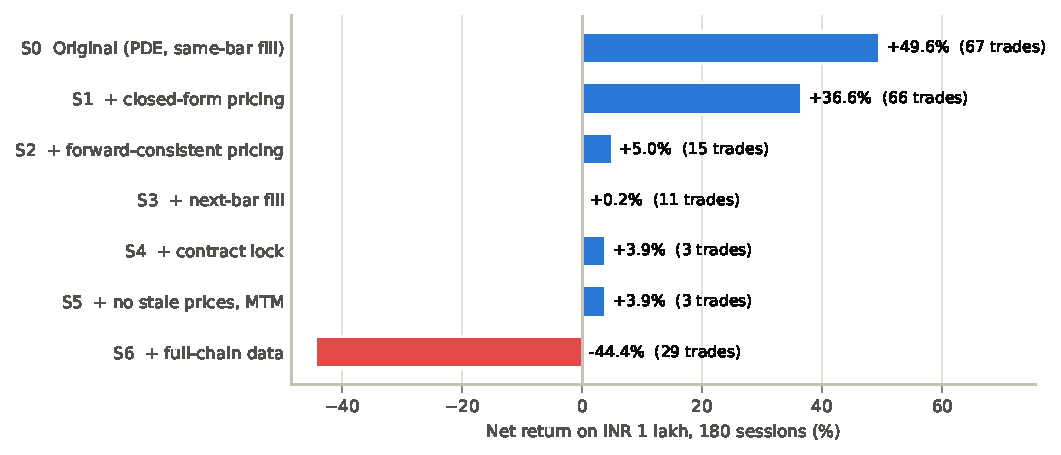
\includegraphics[width=\columnwidth]{fig1_correction_waterfall}
\caption{Net return of the Pure Mispricing strategy on the original 180 sessions as corrections are added cumulatively (Table~\ref{tab:waterfall}).}
\label{fig:waterfall}
\end{figure}

Closed-form pricing removes about a quarter of the headline. Forward-consistent pricing removes nearly all of the rest: once the carry bias is gone, the strategy trades \ForwardTrades{} times instead of \ClosedFormTrades{}, and the return is within noise of zero. Next-bar fills and the contract lock leave $+\LagReturn\%$ and then \LockTrades{} trades, too few to say anything. Row S6 is not a further correction but a change of data. On the full chain with a longer-dated signal expiry, the same rules trade \FullChainDTrades{} times in these sessions and lose $\FullChainDReturn\%$.

% ============================================================================
\section{Corrected Results, 2021--2024}
\label{sec:results}
Each strategy--period cell in Table~\ref{tab:periods} is an independent backtest from INR~1~lakh. Slicing one continuous run is misleading here: Pure and Retail lose most of their capital in 2021, after which the 95\%-of-equity cap blocks or changes later entries. Portfolio returns depend on a few trades and on the capital path, so the table adds statistics that do not: the mean and median net return on premium per trade with a bootstrap 95\% interval \cite{efron1993bootstrap}, the profit factor, and the return without the single largest trade. It also gives the percentile against \RandomDraws{} draws of a random baseline that buys near-ATM puts on the signal expiry with the same fills, exits and costs, with its entry rate calibrated to each strategy's trade count. Because long puts lose to time decay, this baseline usually loses money too, and the comparison is against it, not against zero.

\begin{table*}[!t]
\centering
\scriptsize
\caption{Corrected results, full-chain data, independent backtests from INR 1 lakh in each period.}
\label{tab:periods}
\resizebox{\linewidth}{!}{%
\begin{tabular}{llrrrlrrrrrlr}
\toprule
Period & Strategy & N & Ret \% & Ret ex-max \% & Mean RoP \% [CI] & Med RoP \% & Win \% & PF & Sharpe & MDD \% & Random puts \% [5, 95] & Pctl \\
\midrule
A (2021) & Pure & 40 & -43.0 & -64.5 & -5.2 [-27.2, 21.5] & -37.7 & 28 & 0.65 & -0.85 & 56 & -27.7 [-82, +31] & 34 \\
A (2021) & Hybrid & 23 & +25.7 & +4.3 & 13.2 [-14.3, 44.6] & -14.2 & 43 & 1.47 & 0.78 & 17 & -16.7 [-60, +29] & 93 \\
A (2021) & Retail & 54 & -96.3 & -75.5 & -11.9 [-27.9, 5.6] & -41.1 & 30 & 0.55 & -0.57 & 97 & -39.5 [-95, +22] & 2 \\
\midrule
B (2022) & Pure & 40 & +5.7 & -34.4 & -2.2 [-21.9, 20.4] & -34.1 & 38 & 1.05 & 0.27 & 33 & +3.7 [-63, +74] & 51 \\
B (2022) & Hybrid & 16 & -15.3 & -55.4 & -4.2 [-37.4, 39.5] & -35.0 & 38 & 0.77 & -0.19 & 38 & +1.4 [-52, +59] & 33 \\
B (2022) & Retail & 64 & -17.6 & -41.6 & -1.8 [-17.3, 14.6] & -37.4 & 38 & 0.93 & 0.07 & 46 & -2.2 [-71, +65] & 36 \\
\midrule
C (Jan-Sep 2023) & Pure & 24 & -36.2 & -32.3 & -22.8 [-33.3, -10.4] & -35.9 & 21 & 0.11 & -3.71 & 41 & -16.1 [-42, +11] & 12 \\
C (Jan-Sep 2023) & Hybrid & 10 & -13.1 & -9.9 & -22.6 [-43.3, 5.4] & -42.2 & 20 & 0.25 & -2.17 & 19 & -7.0 [-24, +12] & 27 \\
C (Jan-Sep 2023) & Retail & 44 & -49.3 & -60.2 & -13.4 [-29.3, 4.2] & -41.4 & 30 & 0.58 & -1.17 & 61 & -29.2 [-56, -3] & 13 \\
\midrule
D (Oct 2023-Jun 2024) & Pure & 29 & -44.4 & -9.3 & -6.7 [-24.8, 14.2] & -26.6 & 34 & 0.51 & -1.23 & 52 & -37.3 [-73, +9] & 45 \\
D (Oct 2023-Jun 2024) & Hybrid & 12 & -10.6 & -21.9 & -4.7 [-38.3, 37.5] & -30.6 & 33 & 0.63 & -1.01 & 22 & -16.3 [-51, +22] & 61 \\
D (Oct 2023-Jun 2024) & Retail & 50 & +2.1 & -17.9 & -0.5 [-18.8, 18.4] & -38.3 & 38 & 1.01 & 0.24 & 63 & -63.9 [-93, -27] & 99 \\
\bottomrule
\end{tabular}}
\par\vspace{2pt}
\parbox{\linewidth}{\footnotesize Ret ex-max removes the single trade with the largest absolute P\&L. RoP is net return on premium per trade (bootstrap 95\% CI). PF is profit factor. Random puts: puts-only random entries on the signal expiry with the same fills, exits and costs, entry rate calibrated to the strategy's trade count; mean and 5th--95th percentiles over the draws. Pctl is the strategy's return percentile within that distribution.}
\end{table*}


\begin{figure*}[!t]
\centering
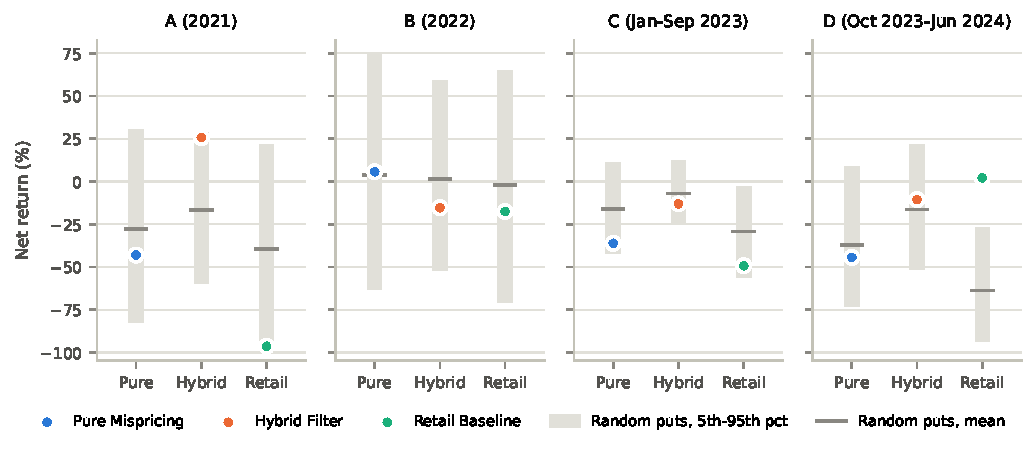
\includegraphics[width=0.9\textwidth]{fig2_period_returns_vs_random}
\caption{Net return of each strategy--period cell (independent backtests from INR~1~lakh) against the matched random-put baseline (5th--95th percentile band and mean).}
\label{fig:periods}
\end{figure*}

Of the 12 cells, \CellsPositive{} are profitable, and the interval for the mean return per trade lies above zero in \CellsCIAboveZero{} of them. In \CellsCIBelowZero{} it lies entirely below zero: Pure Mispricing in Period C, upper bound \PureCRoPHi\%. The cells that look notable rest on single trades. Hybrid's $+\HybridAReturn\%$ in 2021 (\HybridAPctl th percentile of the random baseline) becomes $+\HybridAExMax\%$ without its largest trade. With 12 cells, one return of that size is not unusual under no edge \cite{harvey2016cross}, so we do not treat it as a finding. Retail's $+\RetailDReturn\%$ in Period D ranks at the \RetailDPctl th percentile only because random long puts lost $\RetailDRandomMean\%$ on average in that rising market. Without its largest trade Retail returns $\RetailDExMax\%$.

Pure's $\PureDReturn\%$ in Period D becomes $\PureDExMax\%$ without its largest loss of INR~\PureDLargest. That trade is genuine. The signal fired on \LargestSignalDate{} on the \LargestStrike{} put. The next-bar fill bought it at the close of \LargestEntryDate, the 2024 general-election result day, \LargestDTE{} days before expiry. The index closed $\LargestIndexMove\%$ from the signal close, leaving the put \LargestITM{} points in the money. The fill price of INR~\LargestEntryPrice{} equals the settlement price (INR~\LargestSettle) on \LargestContracts{} contracts, so it is not a stale or erroneous print. The index rebounded and the stop-loss closed the trade on \LargestExitDate{} at INR~\LargestExitPrice. Such fills are the mechanism by which unhedged long options turn a small relative-value signal into large directional outcomes.

\begin{table}[!t]
\centering
\scriptsize
\caption{Trades pooled over the four independent period runs, by option type and exit reason.}
\label{tab:breakdown}
\resizebox{\linewidth}{!}{%
\begin{tabular}{lllrrrrr}
\toprule
Strategy & Type & Exit & N & Net P\&L (INR) & Mean RoP \% & Win \% & Bars \\
\midrule
Pure & put & mean reverted & 48 & -32,191 & -4.3 & 44 & 2.4 \\
Pure & put & stop loss & 65 & -314,214 & -48.2 & 0 & 1.8 \\
Pure & put & take profit & 19 & 212,302 & +118.3 & 100 & 2.1 \\
Pure & put & time expiry & 1 & 16,153 & +51.9 & 100 & 5.0 \\
\midrule
Hybrid & put & mean reverted & 18 & -10,945 & -1.7 & 50 & 2.5 \\
Hybrid & put & stop loss & 30 & -144,468 & -50.1 & 0 & 1.5 \\
Hybrid & put & take profit & 13 & 142,172 & +114.5 & 100 & 2.2 \\
\midrule
Retail & call & pre expiry squareoff & 1 & 129 & +0.7 & 100 & 1.0 \\
Retail & call & stop loss & 46 & -260,746 & -52.1 & 0 & 2.8 \\
Retail & call & take profit & 24 & 273,395 & +93.3 & 100 & 3.2 \\
Retail & call & time expiry & 17 & 28,207 & +11.2 & 71 & 5.0 \\
Retail & put & pre expiry squareoff & 1 & -1,285 & -19.4 & 0 & 3.0 \\
Retail & put & stop loss & 85 & -473,825 & -48.8 & 0 & 2.2 \\
Retail & put & take profit & 30 & 268,050 & +91.5 & 100 & 2.3 \\
Retail & put & time expiry & 8 & 5,027 & +2.1 & 62 & 5.0 \\
\bottomrule
\end{tabular}}
\end{table}


Table~\ref{tab:breakdown} pools the trades of the independent runs. Stop-losses dominate. Pure's stop-loss exits lost INR~\PureStopLossPnL{} against INR~\PureTakeProfitPnL{} won on take-profits, and its mean-reversion exits, the ones the strategy is designed around, lost money on average. By India VIX regime (Table~\ref{tab:vix}), no strategy has a per-trade interval above zero in any regime. With costs scaled up to three times (Table~\ref{tab:stress}), the Pure strategy's interval never lies above zero either.

\begin{table}[!t]
\centering
\scriptsize
\caption{Trade-level results by volatility regime, pooled over the independent period runs.}
\label{tab:vix}
\resizebox{\linewidth}{!}{%
\begin{tabular}{llrlr}
\toprule
India VIX at entry & Strategy & N & Mean RoP \% [CI] & Win \% \\
\midrule
Low VIX ($<$ 12.6) & Pure & 23 & -16.3 [-30.8, 0.8] & 30 \\
Low VIX ($<$ 12.6) & Hybrid & 12 & -10.1 [-34.9, 18.3] & 33 \\
Low VIX ($<$ 12.6) & Retail & 45 & 1.0 [-16.2, 19.8] & 40 \\
\midrule
Normal VIX (12.6 - 14.5) & Pure & 25 & -9.3 [-27.7, 14.1] & 28 \\
Normal VIX (12.6 - 14.5) & Hybrid & 10 & -1.5 [-39.7, 47.3] & 30 \\
Normal VIX (12.6 - 14.5) & Retail & 40 & -8.4 [-28.0, 13.5] & 30 \\
\midrule
High VIX ($>$ 14.5) & Pure & 81 & -5.8 [-20.2, 10.9] & 31 \\
High VIX ($>$ 14.5) & Hybrid & 38 & 0.1 [-21.8, 26.0] & 37 \\
High VIX ($>$ 14.5) & Retail & 126 & -8.2 [-18.9, 3.2] & 33 \\
\bottomrule
\end{tabular}}
\end{table}

\begin{table}[!t]
\centering
\scriptsize
\caption{Pure Mispricing under scaled transaction costs (independent period runs).}
\label{tab:stress}
\resizebox{\linewidth}{!}{%
\begin{tabular}{llrrrrrl}
\toprule
Costs & Entry threshold & N & A \% & B \% & C \% & D \% & Mean RoP \% [CI] \\
\midrule
1.0x & Epsilon fixed & 133 & -43.0 & +5.7 & -36.2 & -44.4 & -7.8 [-18.1, 3.5] \\
1.0x & Epsilon scaled & 133 & -43.0 & +5.7 & -36.2 & -44.4 & -7.8 [-18.1, 3.5] \\
1.5x & Epsilon fixed & 133 & -46.2 & +2.1 & -37.6 & -46.9 & -8.7 [-19.0, 2.6] \\
1.5x & Epsilon scaled & 91 & -35.7 & -21.2 & -20.8 & -41.0 & -5.4 [-18.3, 9.0] \\
2.0x & Epsilon fixed & 133 & -49.4 & -1.5 & -39.1 & -49.4 & -9.7 [-19.9, 1.7] \\
2.0x & Epsilon scaled & 70 & -13.0 & -31.0 & -13.8 & -39.0 & -7.6 [-22.8, 9.7] \\
3.0x & Epsilon fixed & 133 & -55.8 & -8.7 & -41.9 & -54.3 & -11.5 [-21.8, -0.2] \\
3.0x & Epsilon scaled & 47 & -19.3 & -45.9 & -5.1 & -31.6 & -10.0 [-27.4, 10.5] \\
\bottomrule
\end{tabular}}
\par\vspace{2pt}
\parbox{\linewidth}{\footnotesize Epsilon fixed: realised costs scale, the entry threshold does not. Epsilon scaled: both scale.}
\end{table}


% ============================================================================
\section{Testing the Signal Itself}
\label{sec:signal}
A negative backtest of a long-put strategy does not by itself show the mispricing is uninformative. The signal is a relative-value gap, while an unhedged long put adds index direction and time decay that can swamp it. We therefore measure each signal directly. For every near-ATM put on the signal expiry and every session $t$, define the delta-hedged change
\begin{equation}
h_{t \to t+1} = \big(P_{t+1} - P_t\big) - \Delta_F(t)\,\big(F_{t+1} - F_t\big),
\end{equation}
where $\Delta_F$ is Black's put delta with respect to the forward at the surface volatility, and $F = S e^{rT}$ uses the index close rather than the parity forward, so the hedge does not reuse the option prices the signal is built from. $h_{t\to t+1}$ asks whether the gap reverts at all, starting from the signal's own closing price. $h_{t+1\to t+2}$ is what a trader filling at the next close could capture. Because hedged long options lose time value whatever the signal, the relevant quantity is the excess over all near-ATM puts in the same period.

\begin{table*}[!t]
\centering
\scriptsize
\caption{Delta-hedged next-bar P\&L of the put signal, full-chain data (signal expiry $\geq$ 14 DTE).}
\label{tab:signal_v2}
\resizebox{\linewidth}{!}{%
\begin{tabular}{llrllrr}
\toprule
Period & Group & N & $h_{t\to t+1}$ [CI] & $h_{t+1\to t+2}$ [CI] & Excess $h_{t+1\to t+2}$ & Cost \\
\midrule
A (2021) & undervalued & 134 & 4.68 [-3.89, 15.10] & -1.79 [-7.93, 5.39] & +0.29 & 3.50 \\
 & rich & 160 & -10.39 [-15.27, -5.30] & 1.99 [-5.56, 11.91] & +4.07 & 3.27 \\
 & all & 1375 & -3.06 [-5.78, -0.09] & -2.08 [-4.92, 0.95] &  & 3.28 \\
\midrule
B (2022) & undervalued & 113 & 1.66 [-4.44, 8.22] & 2.75 [-3.46, 9.24] & +5.68 & 3.93 \\
 & rich & 145 & -13.32 [-18.36, -8.22] & -4.74 [-9.02, -0.31] & -1.81 & 3.75 \\
 & all & 1464 & -2.85 [-5.81, 0.38] & -2.93 [-5.97, 0.32] &  & 3.89 \\
\midrule
C (Jan-Sep 2023) & undervalued & 42 & -0.15 [-5.82, 5.61] & -3.82 [-9.37, 1.95] & -0.79 & 2.51 \\
 & rich & 70 & -8.72 [-12.84, -4.17] & -5.97 [-9.59, -2.08] & -2.94 & 2.43 \\
 & all & 1102 & -3.13 [-5.22, -0.92] & -3.03 [-5.16, -0.87] &  & 2.66 \\
\midrule
D (Oct 2023-Jun 2024) & undervalued & 63 & 15.96 [-6.46, 48.78] & -0.22 [-9.96, 9.89] & +1.59 & 3.61 \\
 & rich & 52 & -3.92 [-11.70, 5.03] & -5.17 [-12.08, 1.42] & -3.36 & 3.05 \\
 & all & 1054 & -1.17 [-5.16, 2.88] & -1.81 [-5.63, 2.16] &  & 3.24 \\
\midrule
All (2021-2024) & undervalued & 352 & 5.16 [-0.80, 12.73] & -0.28 [-4.02, 3.62] & +2.20 & 3.54 \\
 & rich & 427 & -10.33 [-13.18, -7.44] & -2.47 [-5.94, 1.68] & +0.02 & 3.27 \\
 & all & 4995 & -2.62 [-4.17, -1.02] & -2.48 [-4.03, -0.88] &  & 3.31 \\
\bottomrule
\end{tabular}}
\par\vspace{2pt}
\parbox{\linewidth}{\footnotesize $h$ is the delta-hedged change in the put price per unit (INR): $\Delta P - \Delta_F\,\Delta F$ with the Black-76 forward delta at the surface IV and $F = S e^{rT}$ from the index close. Undervalued: put mispricing $< -\epsilon_t$ (the entry signal); rich: $> +\epsilon_t$. CIs are bootstrap 95\% intervals clustered by date. Excess is the group mean minus the all-puts mean. Cost is the mean round-trip cost per unit.}
\end{table*}


\begin{figure}[!t]
\centering
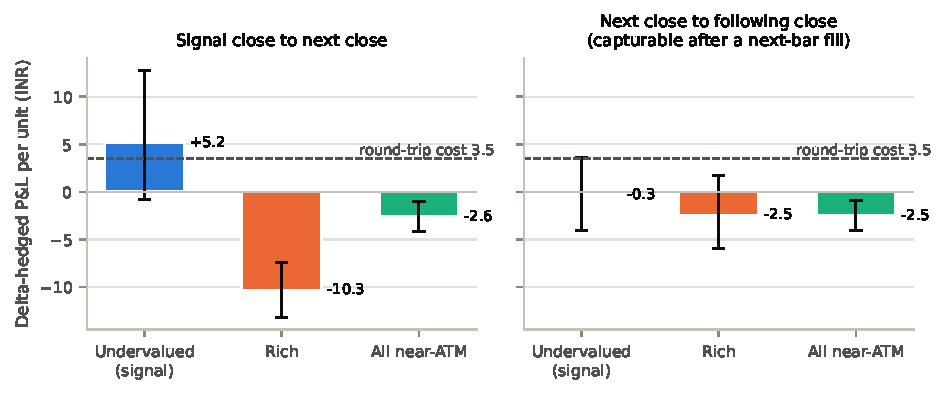
\includegraphics[width=\columnwidth]{fig3_hedged_signal_test}
\caption{Delta-hedged P\&L per unit, all periods pooled, with date-clustered bootstrap 95\% intervals. Left: from the signal close. Right: after a next-bar fill.}
\label{fig:signal}
\end{figure}

Over \SigN{} observations (Table~\ref{tab:signal_v2}, Fig.~\ref{fig:signal}), the signal does contain information. From the signal close to the next close, undervalued puts beat the cross-section by INR~\SigUnderHzeroExcess{} per unit and rich puts trail it by INR~$\SigRichHzeroExcess$. The rank correlation between mispricing and next-day hedged P\&L is $\SigSpearman$. This is the signature of noise in closing prices reverting: a put whose close was low relative to the calls tends to print a more normal price the next day.

The reversion is almost spent by the time a position can be opened. From the next close onward, undervalued puts earn INR~\SigUnderHoneMean{} per unit (interval $[\SigUnderHoneLo, \SigUnderHoneHi]$), an excess of INR~\SigUnderHoneExcess{} over all puts. A round trip costs INR~\SigCost{}. On the legacy one-expiry panel (Table~\ref{tab:signal_legacy}) the ordering of undervalued, rich and all puts is weaker and changes from period to period. The signal is real, but too small and too fast to pay for its own costs at daily frequency.

\begin{table*}[!t]
\centering
\scriptsize
\caption{Delta-hedged next-bar P\&L of the put signal, legacy one-expiry panel (nearest expiry $\geq$ 7 DTE).}
\label{tab:signal_legacy}
\resizebox{\linewidth}{!}{%
\begin{tabular}{llrllrr}
\toprule
Period & Group & N & $h_{t\to t+1}$ [CI] & $h_{t+1\to t+2}$ [CI] & Excess $h_{t+1\to t+2}$ & Cost \\
\midrule
A (2021) & undervalued & 39 & -5.62 [-14.01, 2.92] & -9.66 [-19.90, -2.00] & -1.30 & 3.04 \\
 & rich & 41 & -7.53 [-14.55, 0.37] & -12.72 [-20.35, -2.74] & -4.35 & 2.54 \\
 & all & 958 & -7.85 [-9.85, -5.81] & -8.36 [-10.87, -5.82] &  & 2.65 \\
\midrule
B (2022) & undervalued & 36 & -6.06 [-13.80, 1.82] & -8.38 [-18.26, 2.84] & +1.27 & 2.98 \\
 & rich & 26 & -19.84 [-30.51, -11.04] & -3.45 [-10.56, 4.34] & +6.20 & 2.77 \\
 & all & 878 & -10.09 [-12.52, -7.75] & -9.64 [-12.65, -6.59] &  & 3.05 \\
\midrule
C (Jan-Sep 2023) & undervalued & 11 & -5.38 [-13.38, 11.08] & -11.93 [-19.13, -3.95] & -6.77 & 2.57 \\
 & rich & 22 & -15.26 [-23.88, -5.44] & -12.30 [-16.91, -8.23] & -7.14 & 1.99 \\
 & all & 801 & -6.18 [-8.10, -4.16] & -5.16 [-7.50, -2.77] &  & 2.25 \\
\midrule
D (Oct 2023-Jun 2024) & undervalued & 15 & -16.53 [-35.10, -2.01] & 4.33 [-23.27, 36.38] & +13.91 & 2.59 \\
 & rich & 20 & -13.84 [-30.37, 1.05] & 4.57 [-9.04, 21.14] & +14.14 & 2.64 \\
 & all & 663 & -9.76 [-13.40, -6.31] & -9.57 [-14.09, -5.27] &  & 2.66 \\
\midrule
All (2021-2024) & undervalued & 101 & -7.37 [-12.58, -2.17] & -8.42 [-13.87, -2.94] & -0.38 & 2.90 \\
 & rich & 109 & -13.18 [-18.36, -7.82] & -7.33 [-12.11, -2.27] & +0.71 & 2.50 \\
 & all & 3300 & -8.43 [-9.65, -7.18] & -8.04 [-9.52, -6.54] &  & 2.66 \\
\bottomrule
\end{tabular}}
\par\vspace{2pt}
\parbox{\linewidth}{\footnotesize $h$ is the delta-hedged change in the put price per unit (INR): $\Delta P - \Delta_F\,\Delta F$ with the Black-76 forward delta at the surface IV and $F = S e^{rT}$ from the index close. Undervalued: put mispricing $< -\epsilon_t$ (the entry signal); rich: $> +\epsilon_t$. CIs are bootstrap 95\% intervals clustered by date. Excess is the group mean minus the all-puts mean. Cost is the mean round-trip cost per unit.}
\end{table*}


% ============================================================================
\section{Limitations}
\begin{itemize}
    \item \textbf{Daily closes.} Fills at the daily CLOSE ignore the bid-ask spread beyond the 0.5\% half-spread allowance and intraday timing. Intraday data could show whether the overnight reversion in Section~\ref{sec:signal} is capturable earlier, but it would face the same costs.
    \item \textbf{The surface is still partly circular.} The spline passes through the call implied volatilities, so calls carry no signal by construction. A surface fitted independently of the price being tested (for example leave-one-out across strikes, or a joint fit to calls and puts) is the natural next test. If run on Periods A--C, it must be reported as exploratory, since those periods have now been examined.
    \item \textbf{Fixed rules.} The strike choice (the first qualifying strike in ascending order), $\kappa$, the 150-point window and the stop and target levels were not tuned in this audit, and we deliberately did not adjust them after seeing results. Other choices would give other numbers; changing them to rescue a result would be the selection problem described in \cite{bailey2017probability}.
    \item \textbf{Sizing.} Every trade is 50 units regardless of premium, so expensive in-the-money fills (Section~\ref{sec:results}) carry more risk than cheap ones.
    \item \textbf{Sample.} There are three and a half years, one index and one exchange.
\end{itemize}

% ============================================================================
\section{Conclusion}
The $+\HeadlineReturn\%$ return reported for a PDE mispricing strategy on NIFTY options was produced by finite-difference grid error, a zero-dividend carry bias, same-bar fills, positions marked against the wrong contract, and exit-only accounting. Correcting them on the original sample removes the profit. On a rebuilt full chain over 2021--2024, neither the mispricing strategy, its momentum-filtered variant, nor an RSI/MACD baseline shows a per-trade edge with an interval above zero in any period. Measured directly and hedged, the mispricing does revert overnight, but what remains after a realistic fill is smaller than the cost of trading it.

For practitioners, the lesson is that in a strategy trading model-versus-market gaps, every modelling shortcut becomes a signal. Each one has to be checked against a closed-form or parity benchmark before any backtest is believed. All code, data and the script that regenerates every number in this paper accompany it.

\bibliographystyle{IEEEtran}
\begin{thebibliography}{15}

\bibitem{black1973pricing}
F.~Black and M.~Scholes, ``The pricing of options and corporate liabilities,'' \emph{Journal of Political Economy}, vol.~81, no.~3, pp.~637--654, 1973.

\bibitem{merton1973theory}
R.~C.~Merton, ``Theory of rational option pricing,'' \emph{Bell Journal of Economics and Management Science}, vol.~4, no.~1, pp.~141--183, 1973.

\bibitem{black1976pricing}
F.~Black, ``The pricing of commodity contracts,'' \emph{Journal of Financial Economics}, vol.~3, no.~1--2, pp.~167--179, 1976.

\bibitem{crank1947practical}
J.~Crank and P.~Nicolson, ``A practical method for numerical evaluation of solutions of partial differential equations of the heat-conduction type,'' \emph{Mathematical Proceedings of the Cambridge Philosophical Society}, vol.~43, no.~1, pp.~50--67, 1947.

\bibitem{duffy2006finite}
D.~J.~Duffy, \emph{Finite Difference Methods in Financial Engineering: A Partial Differential Equation Approach}.\hskip 1em plus 0.5em minus 0.4em\relax Hoboken, NJ: John Wiley \& Sons, 2006.

\bibitem{wilmott2006paul}
P.~Wilmott, \emph{Paul Wilmott on Quantitative Finance}, 2nd~ed.\hskip 1em plus 0.5em minus 0.4em\relax Hoboken, NJ: John Wiley \& Sons, 2006.

\bibitem{schwartz1977valuation}
E.~S.~Schwartz, ``The valuation of warrants: Implementing a new approach,'' \emph{Journal of Financial Economics}, vol.~4, no.~1, pp.~79--93, 1977.

\bibitem{li2005superlu}
X.~S.~Li, ``An overview of SuperLU: Algorithms, implementation, and user interface,'' \emph{ACM Transactions on Mathematical Software}, vol.~31, no.~3, pp.~302--325, 2005.

\bibitem{sebi2023study}
SEBI, ``Analysis of Profit and Loss of Individual Traders in Equity Derivatives Segment,'' \emph{Securities and Exchange Board of India Research Report}, January~2023.

\bibitem{bailey2017probability}
D.~H.~Bailey, J.~M.~Borwein, M.~L\'{o}pez de Prado, and Q.~J.~Zhu, ``The probability of backtest overfitting,'' \emph{Journal of Computational Finance}, vol.~20, no.~4, pp.~39--69, 2017.

\bibitem{harvey2016cross}
C.~R.~Harvey, Y.~Liu, and H.~Zhu, ``\ldots and the cross-section of expected returns,'' \emph{Review of Financial Studies}, vol.~29, no.~1, pp.~5--68, 2016.

\bibitem{efron1993bootstrap}
B.~Efron and R.~J.~Tibshirani, \emph{An Introduction to the Bootstrap}.\hskip 1em plus 0.5em minus 0.4em\relax New York: Chapman \& Hall, 1993.

\bibitem{wilder1978new}
J.~W.~Wilder, \emph{New Concepts in Technical Trading Systems}.\hskip 1em plus 0.5em minus 0.4em\relax Greensboro, NC: Trend Research, 1978.

\bibitem{appel2005technical}
G.~Appel, \emph{Technical Analysis: Power Tools for Active Investors}.\hskip 1em plus 0.5em minus 0.4em\relax Upper Saddle River, NJ: FT Press, 2005.

\end{thebibliography}

\end{document}
